% Great thanks for Cezary Sałbut (this latex file is mainly based on his work)

\documentclass[a4paper,12pt,fleqn]{article}


\usepackage[utf8]{inputenc} 
\usepackage{polski}
\usepackage[polish]{babel}
\usepackage[pdftex]{color,graphicx}
\usepackage{subfig}
\usepackage{indentfirst}
\usepackage{booktabs}
\usepackage{tabularx}
\usepackage{multirow}
\usepackage{pdflscape}
\usepackage{array}
\usepackage{amsmath}
\usepackage{appendix}
\usepackage{hyperref}
\hypersetup{
    colorlinks,%
    citecolor=black,%
    filecolor=black,%
    linkcolor=black,%
    urlcolor=blue
}

\usepackage{listings}
\lstset{
	numbers=left, 
	stepnumber=1, 
	basicstyle={\footnotesize \ttfamily},
	language=C, 
	captionpos=b,
	xleftmargin=6mm,
	aboveskip=\medskipamount,
	belowskip=\bigskipamount,
	tabsize=4
}

\usepackage{title-page}

\usepackage[top=28mm, bottom=30mm, left=21mm, right=21mm]{geometry}

\linespread{1.5}		%interlinia

\usepackage{boxedminipage} 
%% change the below lengths to suit your needs: 
\setlength{\fboxrule}{1pt} 
\setlength{\fboxsep}{5pt}



\renewcommand{\appendixtocname}{Dodatki}
\renewcommand{\appendixpagename}{Dodatki}


\widowpenalty=10000
\clubpenalty=10000


\newcommand{\autor}{Jan Kurdel}
\newcommand{\tytulpl}{Identyfikacja nieliniowych obiektów dynamicznych metodą uogólnionej regresji postępującej z ortogonalizacją}
\newcommand{\tytulen}{Identification of nonlinear dynamical objects based on Generalized Orthogonal Forward Regression}
\newcommand{\uczelnia}{POLITECHNIKA WARSZAWSKA}
\newcommand{\wydzial}{Wydział Elektroniki i Technik Informacyjnych}
\newcommand{\instytut}{Instytut Systemów Elektronicznych}
\newcommand{\promotor}{dr inż. Stanisława Jankowskiego}
\newcommand{\praca}{Praca inżynierska}
\newcommand{\miejscerok}{Warszawa, 2012}
\newcommand{\indeks}{214460}

\title{\tytulpl}
\author{\autor}

\begin{document}

\renewcommand{\tablename}{Tabela}

\pagestyle{empty}
\stronatytulowa

\newpage
\setcounter{page}{1}

\newpage
\tableofcontents

\newpage
\pagestyle{plain}

\section{Równania różniczkowe zwyczajne}

Równaniem różniczkowym zwyczajnym nazywamy równanie zawierające zmienną niezależną $x$, nieznaną funkcję $y$, oraz jej pochodne $y', y'', \hdots, y^{(n)}$ \cite[str. 7]{BCh_2001}
\begin{equation}
	\label{wzor:rownanie_roz_N_stopnia}
	F(x,y,y',\hdots,y^{(n)}) = 0
\end{equation}
gdzie $F:R^{n+2} \rightarrow R$

Warunek początkowy (Cauchy'ego) dla równania \ref{wzor:rownanie_roz_N_stopnia} określony jest poprzez: 

\begin{equation}
\begin{array}{c}
y(x_0)       =  y_0,     \\
y'(x_0)      =  y_1,     \\
\vdots			   	     \\
y^{n-1}(x_0) = y_{n-1}
\end{array}
\end{equation}
gdzie $y_0, y_1, \hdots, y_{n-1}$ są zadanymi liczbami.

Stopień pochodnej w równaniu \ref{wzor:rownanie_roz_N_stopnia} decyduje o rzędzie równania różniczkowego. Równanie różniczkowe pierwszego rzędu wyraża się zatem wzorem:
\begin{equation}
	\label{wzor:rownanie_roz_I_stopnia}
	y' = f(x,y)
\end{equation}

Rozwiązanie równania \ref{wzor:rownanie_roz_I_stopnia} w sposób numeryczny może zostać rozwiązane z wykorzystaniem wielu sposobów. Można wyróżnić podział na metody jednokrokowe, które wymagają jedynie informacji z poprzedniego kroku (zatem warunek początkowy jest wystarczający do obliczenia równania różniczkowego dla kolejnego punktu) oraz metody wielokrokowe, w których rozwiązanie jest dokonowywane z wykorzystaniem znajomości kilku poprzednich kroków. Wśród metod jednokrokowych znajdują się m.in. metody Eulera oraz Rungego-Kutty.

\subsection*{Metoda Eulera}
Metoda Eulera jest najprostszą metodą numeryczną rozwiązywania równań różniczkowych. Mając dane równanie \ref{wzor:rownanie_roz_I_stopnia} oraz warunek początkowy postaci:
\begin{equation}
	y(x_0) = y_0	
\end{equation}
poszukujemy rozwiązania dla kolejnego momentu $x_1 = x_0 + h$ gdzie $h$ jest krokiem metody. W tym celu możemy skorzystać z rozwinięcia szeregu Taylora w pobliżu punktu początkowego $x_0$:
\begin{equation}
	y(x_0 + h) = y(x_0) + hy'(x_0) + \frac{h^2}{2!}y''(x_0) + \hdots
\end{equation}
Korzystając tylko z dwóch pierwszych elementów szeregu Taylora otrzymamy:
\begin{equation}
	y(x_0 + h) = y(x_0) + hy'(x_0) = y(x_0) + hf(x_0,y_0)
\end{equation}
Powtarzając tę czynność wielokrotnie otrzymamy wzór:
\begin{equation}
	y_{n+1} = y_{n} + hf(x_n,y_n)
\end{equation}
określany jawną metodą Eulera.

\subsection*{Metoda Rungego-Kutty}
Kolejną metodą numerycznego rozwiązywania równań różniczkowych jest metoda Rungego-Kutty, która jest metodą wieloetapową. W każdym kroku konieczne jest obliczenie wartości funkcji $f$ dla różnych argumentów. Wśród metod Runge-Kutty można wyróżnić różne metody w zależności od rzędu metody. Najprostszą z nich jest metoda Runge-Kutty rzędu II. Przyjmuje ona postać:
\begin{equation}
	y_{i+1} = y_i + \frac{h}{2}(k_1 + k_2)
\end{equation}
gdzie
$$\begin{array}{c}
	k_1 = f(t_i,y_i) \\
	k_2 = f(t_i + h, y_i + hk_1)
\end{array}$$

Najbardziej popularną jest metoda rzędu IV, która przyjmuje postać:
\begin{equation}
	y_{i+1} = y_i + \frac{h}{6}(k_1 + 2k_2 + 2k_3 + k_4)
\end{equation}
gdzie
$$\begin{array}{c}
	k_1 = f(t_i,y_i) \\
	k_2 = f(t_i + \frac{h}{2}, y_i + \frac{h}{2}k_1) \\
	k_3 = f(t_i + \frac{h}{2}, y_i + \frac{h}{2}k_2) \\
	k_4 = f(t_i + h,y_i + hk_3) \\
\end{array}$$

\subsection*{Równania różniczkowe zwyczajne wyższych rzędów}
Równanie różniczkowe wyższych rzędów może zostać sprowadzone do układu równań różniczkowych rzędu pierwszego \cite[str. 293]{AK_RBG2002}. Mając dane równanie różniczkowego n-tego rzędu:
$$y^{(n)}(t) = f(t,y(t),y'(t),\hdots,y^{(n-1)}(t)), \qquad a \leq t \leq b$$
z warunkiem początkowym w postaci:

$$\begin{array}{c}
y(a)       = \alpha_0,    \\
y'(a)      = \alpha_1,    \\
\vdots					  \\
y^{n-1}(a) = \alpha_{n-1} \\
\end{array}$$

oraz wprowadzając nowe zmienne:
$$y_1(t) = y(t), y_2(t) = y'(t), \hdots, y_n(t) = y^{(n-1)}(t)$$

otrzymujemy układ równań różniczkowych pierwszego rzędu postaci:
$$\begin{array}{l}
y'_1       = y_2   \\
y'_2       = y_3   \\
\vdots			   \\
y'_{n-1} = y_n     \\
y'_n = f(t,y_1,y_2,\hdots,y_n)
\end{array}$$

z warunkami początkowymi postaci:
$$y_1(a) = \alpha_0, y_2(a) = \alpha_1, \hdots, y_n(a) = \alpha_{n-1}$$

Dzięki takiemu zabiegowi możliwe jest rozwiązanie równania różniczkowego wyższego rzędu metodami służącymi do rozwiązywania równań różniczkowych rzędu pierwszego.

\newpage
\section{Sieci neuronowe}
Sieci neuronowe powstały \textbf{opisać jak powstały}. Podstawą budowy sieci neuronowych są neurony. Budowa pojedynczego neuronu jest przedstawiona na rysunku \ref{fig:neuron}. Neuron taki sumuje sygnał podany na jego wejścia $x_i$ z odpowiednimi wagami $w_i$, dając na wyjście wynik $y$ sumy przeprowadzonej przez funkcję aktywacji $f(x)$.
\begin{figure}[ht!]
	\centering
	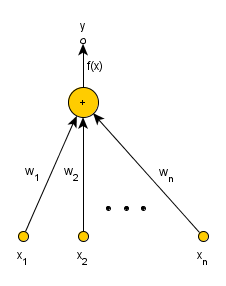
\includegraphics[scale=0.8]{images/single_neuron.png}
	\caption{Budowa pojedynczego neuronu}
	\label{fig:neuron}
\end{figure}

Sieć neuronową budują grupy połączonych ze sobą neuronów. Strukturę sieci wielowarstwowej przedstawia rysunek \ref{fig:neuron} \textbf{ZMienić rysunek}. Pierwsza warstwa nosi nazwę warstwy wejściowej, ostatnia warstwa sieci nosi nazwę warstwy wyjściowej. Wszystkie pozostałe warstwy noszą nazwę warstwy ukrytej.

\subsection*{Sieć RBF}
Sieć RBF (Radial Basis Function) jest sztuczną siecią neuronową o radialnych funkcjach bazowych. Sieć taka składa się zazwyczaj z jednej warstwy ukrytej, gdzie funkcja aktywacji jest radialną funkcją bazową oraz 
warstwy wyjściowej w postaci neuronu liniowego. Radialna funkcja bazowa jest określona w sposób następujący\cite[str. 1]{Bartkowiak}
\begin{equation}
	G(x,c) = G(r(x,c))
\end{equation}
gdzie $r(x,c)$ jest odległością między punktami $r$ i $c$ a centrum $c$ jest ustalone i pełni rolę parametru funkcji. Jedną z bardziej popularnych radialnych funkcji bazowych jest funkcja Gaussa:
\begin{equation}
	G(x,\sigma,c) = e^{\frac{-(x-c)^2}{2\sigma^2}}
\end{equation}
\textbf{Dlaczego taka sieć jest fajna i kiedy się ją stosuję}


\newpage
\section{Metody gradientowe}
Do najbardziej skutecznych metod uczenia sieci neuronowych należą metody gradientowe. Algorytmy te bazują na rozwinięciu w szereg Taylora funkcji celu $E(W)$ w najbliższym sąsiedztwie znanego rozwiązania\cite[str. 54]{Osowski}.
\begin{equation}
	\label{wzor:metoda_gradientowa}
	E(w + p) = E(w) + [(g(w)]^Tp + \frac{1}{2}p^TH(w)p + \hdots
\end{equation}
gdzie
$$g(w) = \nabla E = [\frac{\partial E}{\partial w_1}, \frac{\partial E}{\partial w_2}, \hdots, \frac{\partial E}{\partial w_n}]^T$$
$$H(w) = \begin{bmatrix}
\frac{\partial^2 E}{\partial w_1 \partial w_2} & \hdots & \frac{\partial^2 E}{\partial w_1 \partial w_n}\\
\vdots & & \vdots \\
\frac{\partial^2 E}{\partial w_n \partial w_1} & \hdots & \frac{\partial^2 E}{\partial w_n \partial w_n}
\end{bmatrix}$$
$\nabla E$ jest wektorem pierwszych pochodnych - gradientem, natomiast $H(w)$ jest macierzą drugich pochodnych - hesjanem. W praktyce są używane co najwyżej 3 pierwsze elementy równania~\ref{wzor:metoda_gradientowa}. W metodzie gradientowej poszukuje się minimum funkcji celu poprzez taką aktualizację wektora kierunkowego $p$ oraz kroku $\eta$ aby prawdziwa była nierówność $E(w_{k+1}) < E(w_k)$.

\subsection*{Algorytm Levenberga-Marquardta}
Podczas gdy wcześniej nie została określona konkretna funkcji celu, tak w przypadku algorytmu Levenberga-Marquardta funkcją celu jest błąd średniokwadratowy (sum-of squares error, Mean Squared Error, MSE)\cite[str. 290]{Bishop}.
\begin{equation}
	\label{wzor:mse}
	E = \frac{1}{2} \sum_1^n(e_n)^2 = \frac{1}{2} \sum_1^n(y_n - \tilde{y_n})^2
\end{equation}
gdzie $e_n$ jest błędem n-tego wzorca, $y_n$ n-tym wzorcem, $\tilde{y_n}$ wyjściem sieci dla n-tego wzorca.

Zakładając, że aktualnie jesteśmy w punkcie $w_{old}$ i chcemy przemieścić się do punktu $w_{new}$, który jest niedaleko oddalony od $w_{old}$ w celu obliczenia nowej wartości $e$ możemy skorzystać z rozwinięcia w szereg Taylora:
\begin{equation}
	\label{wzor:blad_lm}
	e(w_{new}) = e(w_{old}) + Z(w_{new} - w_{old})
\end{equation}
gdzie $Z \equiv \nabla e$. Po podstawieniu równania \ref{wzor:blad_lm} do równania \ref{wzor:mse} wzór na błąd średniokwadratowy może zostać zapisany jako:
\begin{equation}
	\label{wzor:mse2}
	E = \frac{1}{2}(e(w_{old}) + Z(w_{new} - w_{old}))^2
\end{equation}
Chcą zminimalizować równanie \ref{wzor:mse2} ze względu na zmienną $w_{new}$ otrzymujemy wzór na $w_{new}$:
\begin{equation}
	w_{new} = w_{old} - (Z^TZ)^{-1}Z^Te(w_{old})
\end{equation}
Jednak taki sposób obliczania $w_{new}$ może powodować, że krok $w_{new} - w_{old}$ będzie duży a wtedy liniowa aproksymacja szeregiem Taylora może stać się niedokładna. Z tego powodu algorytm Levenberga-Marquardta korzysta ze zmodyfikowanej funkcji celu w postaci:
\begin{equation}
	\label{wzor:mse_lm}
	E = \frac{1}{2}(e(w_{old}) + Z(w_{new} - w_{old}))^2 + \lambda (w_{new} - w_{old})^2
\end{equation}
Chcą zminimalizować równanie \ref{wzor:mse_lm} ze względu na zmienną $w_{new}$ otrzymujemy ostatecznie równanie opisujące sposób obliczania wag w kolejnych iteracjach dla algorytmu Levenberga-Marquardta:
\begin{equation}
	w_{new} = w_{old} -(Z^TZ + \lambda I)^{-1}Z^Te(w_{old})
\end{equation}
gdzie $I$ jest macierzą jednostkową. \textbf{Opisać $\lambda$}



\newpage
\section{Selekcja funkcji bazowych oparta o Orthogonal Least Square}
Jedną z metod selekcji najbardziej znaczących funkcji bazowych jest metoda oparta o metodę najmniejszych kwadratów oraz ortogonalizację \cite{Chen}. Metoda ta umożliwia określenie wkładu każdej funkcji bazowej i wybranie tych najbardziej istotnych. Mając dany wektor wag sieci $w = [w_0, w_1, \hdots, w_K]^T$ oraz wektor danych uczących $d = [d_1, d_2, \hdots, d_p]^T$ można zapisać macierz G w postaci:

\begin{equation}
G = \begin{bmatrix}
\phi_{11} & \phi_{21} & \hdots & \phi_{K1} \\
\phi_{12} & \phi_{22} & \hdots & \phi_{K2} \\
\hdots    & \hdots    & \hdots & \hdots    \\
\phi_{1p} & \phi_{2p} & \hdots & \phi_{Kp}
\end{bmatrix}
\end{equation}

gdzie $\phi_{ji}$ oznacza odpowiedź i-tej funkcji radialnej na j-ty wzorzec uczący. Oznaczając przez $g_i = [g_{i1}, g_{i2}, \hdots, g_{ip}]^T$ odpowiedź i-tej funkcji radialnej na wszystkie wzorce uczące można macierz G przedstawić w postaci:

\begin{equation}G = [g_1, g_2, \hdots, g_K] \end{equation}

Wprowadzając takie oznaczenia można zapisać następujące równanie:
\begin{equation}d = Gw + e\end{equation}

gdzie $e$ jest błędem niedopasowania sieci.
\begin{equation}G = QA\end{equation}

\begin{equation}
A = \begin{bmatrix}
1      & a{12}  & a{13}  & \hdots & a_{1K} \\
0      & 1      & a{23}  & \hdots & a_{2K} \\
\hdots & \hdots & \hdots & \hdots & \hdots \\
0      & 0      & 0      & 0      & 1     
\end{bmatrix}
\end{equation}

No a teraz ortogonalizacja. I ortogonalizacja może być dokonana różnymi metodami z czego jedną z nich jest ortogonalizacja Gramma-Schmidta.

Ortogonalizacji macierzy G można dokonać różnymi metodami z czego jedną z nich jest ortogonalizacja Gramma-Schmidta. \textbf{Opisać teraz metodę Gramma-Schmidta}.


% -------------------------- bibliografia ----------------------------
\newpage

\begin{thebibliography}{widest-label}
\bibitem{AK_RBG2002}Kharab A., Ronald B. Guenther, An introduction to numerical methods : a MATLAB approach, 2002, Chapman \& Hall/CRC

\bibitem{BCh_2001}Bogdan Choczewski (red.), Równania różniczkowe zwyczajne i cząstkowe. Zadania z matematyki, Kraków 2001, Wydawnictwa AGH

\bibitem{Osowski}Osowski S., Sieci neuronowe do przetwarzania informacji, Warszawa 2006, Oficyna Wydawnicza Politechniki Warszawskiej

\bibitem{Bishop}Bishop C. M., Neural Networks for Pattern Recognition, Oxford University Press, 1995 Oxford

\bibitem{Bartkowiak} Bartkowiak A., (Notatki do wykładu Sieci Neuronowe), Sieci RBF - o radialnych funkcjach bazowych, https://www.ii.uni.wroc.pl/~aba/teach/NN/w9rbf.pdf

\bibitem{Chen} Chen S., Cowan C. F. N., Grant P. M., Orthogonal Least Squares Learning Algorithm for Radial Basis Function Networks, IEEE, 1991

\end{thebibliography}

\end{document}
